\section{Link Budget}
Astrea constellation main satellite must be able to stablish three different telecommunications link: 
\begin{itemize}
\item Space to Ground link for payload and TT\&C data.
\item Space to Space link between Astrea satellites.
\item Space to Space link between client and Astrea satellites.
\end{itemize} 

\subsection{Link Budget Calculation}

\subsubsection{Methodology}
From the expected requirements fixed on the Project Charter, general radio systems parameters will computed, in order to have a reference to look for the best communications system on board the Astrea satellites. As background, general losses parameters had been calculated on previous sections. 

The most important concern on AstreaSAT link Budget is how far every satellite can emit on the desired frequencies. This is a key factor to know the utility of the modules selected. At least, Project Charter communication requirements must be accomplish.
 
To verify communication system chosen options, let's start calculating the minim required sensitivity for receiving strong enough signal. With this value, it is possible to know how far the satellite can listen to information.
Applying equation \ref{Appendix:Structure} and equation \ref{Appendix:Structure} on a simple Matlab routine:

\begin{figure}[H]
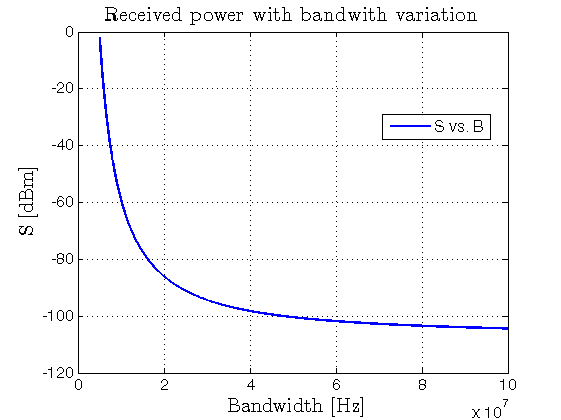
\includegraphics[scale=0.9]{./sections/SatelliteDept/sections/images/SvsB}
\centering
\caption{Sensibility change along Bandwidth variation}
\label{SvsB}
\end{figure}

As bandwidth increments, Sensitivity decrements, meaning that we need higher powered receivers in order to sense high bandwidth communications.

\subsubsection{Range calculation}
To know how far the satellite can be received or listen to, Friis equation \ref{friisEq} will be applied.
 
\begin{equation}
	P_r=P_t+G_t+G_r -FSL -L_{abs}-L_{aml}-L_{point}
	\label{friisEq}
\end{equation}

\begin{align*}
		P_r&:\text{Received power}\\
		P_t&:\text{Transmitted power}\\
		G_t&:\text{Transmitter antenna gain}\\
		G_r&:\text{Receiver antenna gain}\\
		L_{prop}&:\text{All kind of losses}\\
		L_{prop}&=FSL -L_{abs}-L_{aml}-L_{point}  	
\end{align*}

\begin{figure}[h]
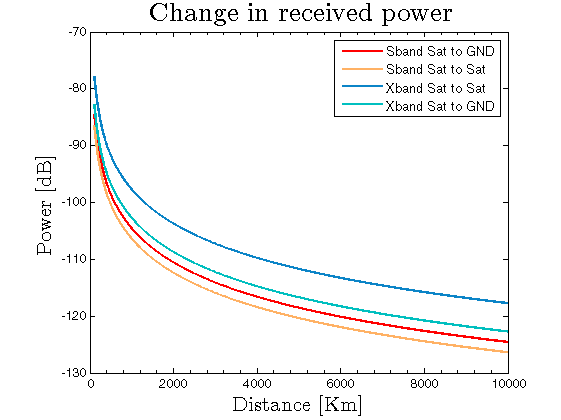
\includegraphics[scale=0.9]{./sections/SatelliteDept/sections/images/friisCases}
\centering
\caption{Received power with distance variation}
\label{friis}
\end{figure}

\subsubsubsection*{S band range}
On Fig.\ref{friis} earth atmosphere and multiple losses (described previously) affect to the received power on ground. Despite all, ground station have powerful antennas that mitigate the losses effect. Therefore, because of the low gain of the antennas between satellites, the link is weaker.

\subsubsubsection*{X band range}
In this case, X band, because its high frequency is more affected by atmospheric losses. Is it possible to appreciate it on Fig.\ref{friis}. Link between satellites is stronger that the one with the ground. Finally remark a fact, despite higher frequencies should have weaker links, in this case, the high antenna gains for X band, confer stronger links to the X band.

In order to use satellite communications, will be necessary to use Fig.\ref{Appendix:Structure} and \ref{friis}. From \ref{friis}, given a determinate altitude a power sensibility can be extract. Then, on \ref{Appendix:Structure}, taking the previous sensibility calculated, a Bandwidth for operation can be stated. The procedure works on both sites.